\documentclass{letter}
\usepackage[top=0.5cm, bottom=0.5cm]{geometry}
\usepackage{pdfpages}
% Set page margins
%\usepackage[left=1in, right=1in, bottom=0.7in, top=0.7in]{geometry}


%\usepackage{wrapfig}

\usepackage[style=ieee, sorting=ydnt]{biblatex} % instead of bibtex; sorts them in reverse chronological order: ydnt
\addbibresource{Tex_publications_since2002.bib}


% Package imports
\usepackage{setspace, longtable, graphicx, hyphenat, hyperref, fancyhdr, ifthen, everypage, enumitem, amsmath, setspace, wrapfig}

% --- Page layout settings ---

% Set line spacing
\renewcommand{\baselinestretch}{1.15}

% --- Page formatting ---

% Set link colors
\usepackage[dvipsnames]{xcolor}
\hypersetup{colorlinks=true, linkcolor=RoyalBlue, urlcolor=RoyalBlue}

% Set font to Libertine, including math support
\usepackage{libertine}
\usepackage[libertine]{newtxmath}

%\usepackage{lipsum}

\address{\\ \\ \\ \large \textbf{Branch of} \\ \large \textbf{
Oral and Maxillofacial Surgery} \\ Wan-Fang Hospital,\\ Taipei Medical University \\}
\date{}


% Chinese
\usepackage{xeCJK} % for Chinese, compiling by XeLaTex
\usepackage{indentfirst}
\setlength{\parindent}{2em}  % setting the indentation to be two Chinese characters size.
\usepackage{fontspec} %設定字體
% Fandol font (the default)  not shown "內"
\setCJKmainfont{AR PL UMing TW MBE} % AR PL UMing TW MBE or "UKai" https://www.overleaf.com/learn/latex/Questions/Which_OTF_or_TTF_fonts_are_supported_via_fontspec%3F#Chinese
%BiauKai} %標楷體 from macOS %設定中文為系統上的字型,而英文不去更動,使用原TeX字型
%\setCJKmainfont[Vertical=RotatedGlyphs]{AR PL UMing TW MBE}


\begin{document}
\begin{letter}
{
\centering \Large \textbf{Letter of Recommendation}
}

\hfill
\begin{wrapfigure}[1]{l}{0.65\linewidth}%{height=0.65\textheight}
    %\centering
    
\includegraphics[width=0.3\textheight]{TMWH.png}
\end{wrapfigure}

\opening{Dear 吳木榮老師}%To Whom it May Concern:} % admissions officer
% 吳木榮 講師 法醫牙科學、法醫病理學
%分機:65507
%ntuhmzw@gmail.com
\medskip 

%Dr. Sun Yihua, ,天資聰穎
\indent 祁力行醫師,受到父親的影響,考取醫學院後,對大學時代的三門課程「大體解剖、電腦概論、法醫學概論」,有著深刻的印象。
自見習時期起,對口腔顎面外科深感興趣,以成為「真正的醫師」為己任。歷經實習、二年期的一般住院醫師訓練後,進入口外專科訓練長達四年,堅韌卓絕,親力親為,不辭勞苦,全年無休天天準時查房,守護患者,遵從主治醫師教導。即使感冒生病,在病房接受點滴注射後,第二天依舊打起精神執行口腔癌手術。在2003臺灣疫情大起之時,家有高堂,仍必須堅守崗位,在危機中協助口腔顎面外科安然渡過難關。

%During his residency training, Dr. Chi Li-Hsing, a talented and intelligent doctor, developed a strong interest in oral and maxillofacial surgery and made it his aim to become a "real doctor."
%He is tenacious, engaged, and hardworking, with 3.5 years of speciality training in oral and maxillofacial surgery.
%He guards patients and rounds the ward at 7:30 a.m. every day of the year, 24 hours a day, 365 days a year, and follows the attending physician's instructions. He was energized to undergo oral cancer surgery the next morning after receiving an intravenous injection in the ward, despite having a cold.
%Although his family's concerns, when the SARS epidemic broke out in Taiwan in 2003, he remained at his post and help the oral and maxillofacial surgery in the crisis.

%In 2009, he volunteered for about three years at Taiwan Medical Mission (in Africa) in compliance with Taipei Medical University policy. Seeing countries with very different norms and customs has made him realize how important it is for doctors and patients to have a pure engagement. He went back to school after returning to Taiwan early 2012 in order to discover a question. He completed a two-year master's program in biomedical informatics in which he has learnt useful information technology before enrolling in a doctoral program in translational medicine. He further completed seven years of graduate studies with the guidance and encouragement of faculty from Taipei Medical University and Academia Sinica, and even during the COVID-19 outbreak of 2021. In terms of the search answer, it has progressively acquired reality.

於2009年,他配合臺北醫學大學政策,奉派至非洲醫療團長駐近三年。見識到風土民情絕然不同的國家,更體認到純真的醫病關係。2012返臺後,重新回到學校,因為他想尋找一個答案。二年的醫學資訊學碩士班,學習到良好的數位工具,接著逕讀轉譯醫學博士班,在北醫與中研院老師的指導與激勵之下,也在2021 COVID-19疫情之下,完成了九年的研究所學業。至於那個尋找中的答案,也逐漸成形。

% https://quillbot.com/
%When he was studying in the doctoral program, he recalled the spirit of forensic medicine 25 years ago, and took the initiative to attend the forensic medicine course in the university.
%He also practiced interpreting the judgments of major criminal cases, and the judicial examination reports in them made him very fascinated by the important role of expert witnesses.
%At that time, his father suffered a stroke and was bedridden, which made him realize the limit of medical care for physical diseases, and turned to pay more attention to spiritual growth and its impact on physical health. Traditional Chinese medicine has many unique insights on this part.

就讀博士班時,憶起25年前的法醫魂,主動旁聽大學部法醫學的課程,也練習解讀重大刑案的判決書,其中的司法相驗報告,讓他對專家證人的重要角色非常神往。
適時也遭逢父親中風臥床的變故,讓他體會到醫學照顧與身體疾病的極限,轉而重視心靈成長,及其對身體健康的影響,中醫對這部分有許多獨到的見解。

於臨床的體晤中,他發現醫學需要謙虛,在科學研究的生涯中,更肯定了全人照護對身心靈與社會關係的全方面影響。他漸漸知道,僅限於分子化學與身體的結構,仍不足以解釋疾病(特別是癌症)會不斷地復發。
於十個月的口腔顎面外科主任的歷練中,他知道醫學教育身教的重要,屢屢發現人性的弱點,並提醒醫療處置必須加強的地方。 % photodynamic therapy
面對生與死的議題,讓他參加「預立醫療意願」的諮商醫師訓練,靈性關懷師的訓練更讓他熟悉全人照顧的方法。

接下來,憑藉著對法醫學的熱誠,以醫師科學家的根底,他要接受挑戰,圓一個法醫師的夢,通過國家法醫師的考試,稟持科學精神,以追求真相為目標,讓逝者得以安心,更讓他們親愛的家人,得以放心,跨過死亡的界線,完整了由生到死的全人照護。
感謝親愛的母親與妻子,全力支持力行的決定,得以投身法醫師的行列,成為「醫師中的醫師」,一向敦促力行要正直的父親,相信在天上一定是非常讚許的。

% 對法醫的工作有興趣、有服務的心態、人夠正直且家裡願意支持,較有機會。
% issue the death certificate at home; manner of the death

綜合上述,玆推薦祁力行醫師,符合法醫學生的資格,以他的勇氣和決心,投身法醫師的行列,寄望能於法醫研究所老師們的指導之下,進修法醫學程及法醫實習,完成法醫師專技高考,以符合社會期許,與他父親的期望,在未來的日子,回到他的初衷,繼續著服務人群的使命。
%茲推薦祁力行醫師,符合法醫學生的資格,有著無比的勇氣和決心,投身法醫師的行列。祁許在未來的日子,回到他的初衷,完成自己的使命。
%It is suggested that Dr. Chi satisfy the requirements and be nominated for Professor Yin Niande's Outstanding Rookie Award, which is well-deserved, with the hope that in her future career as a specialist, he will continue to follow his original aim of serving the welfare of patients.

\medskip
%Sincerely, \\ 
以上報告\\

萬芳醫院口腔顎面外科主任 \hspace{3mm}
祁力行敬上 \hspace{5mm} \today

%Chi, Li-Hsing Tex \\
%Director of OMS, TMWH

\clearpage

%
% Remove page numbering
%\pagenumbering{gobble}

% --- Document starts here ---

%\begin{document}

% Name and date of last update to this document
\noindent{\Huge{Li-Hsing Tex Chi, D.D.S., Ph.D.}
\hfill{\it\footnotesize Updated \today}}

% --- Contact information and other items ---

\vspace{0.5cm} 
\begin{center}
\begin{tabular}{lll}
% Line 1: Email, GitHub, office location
\textbf{Email}: d622101005@tmu.edu.tw      &
\hspace{0.2cm} \textbf{GitHub}: /github.com/texchi2    &
\hspace{0.2cm} 	\textbf{Office}: TMWH \\

% Line 2: Phone number, LinkedIn, citizenship
\textbf{Phone}: +886 970746852   & 
\hspace{0.2cm} \textbf{ResearchGate}: 
/profile/Li\_Hsing\_Chi &
%LinkedIn: /in/tex-chi-073523/   & 
\hspace{0.2cm} \textbf{Citizenship}: Taiwan 
\end{tabular}
\end{center}

\begin{wrapfigure}{r}{0.3\textwidth}
    \centering
    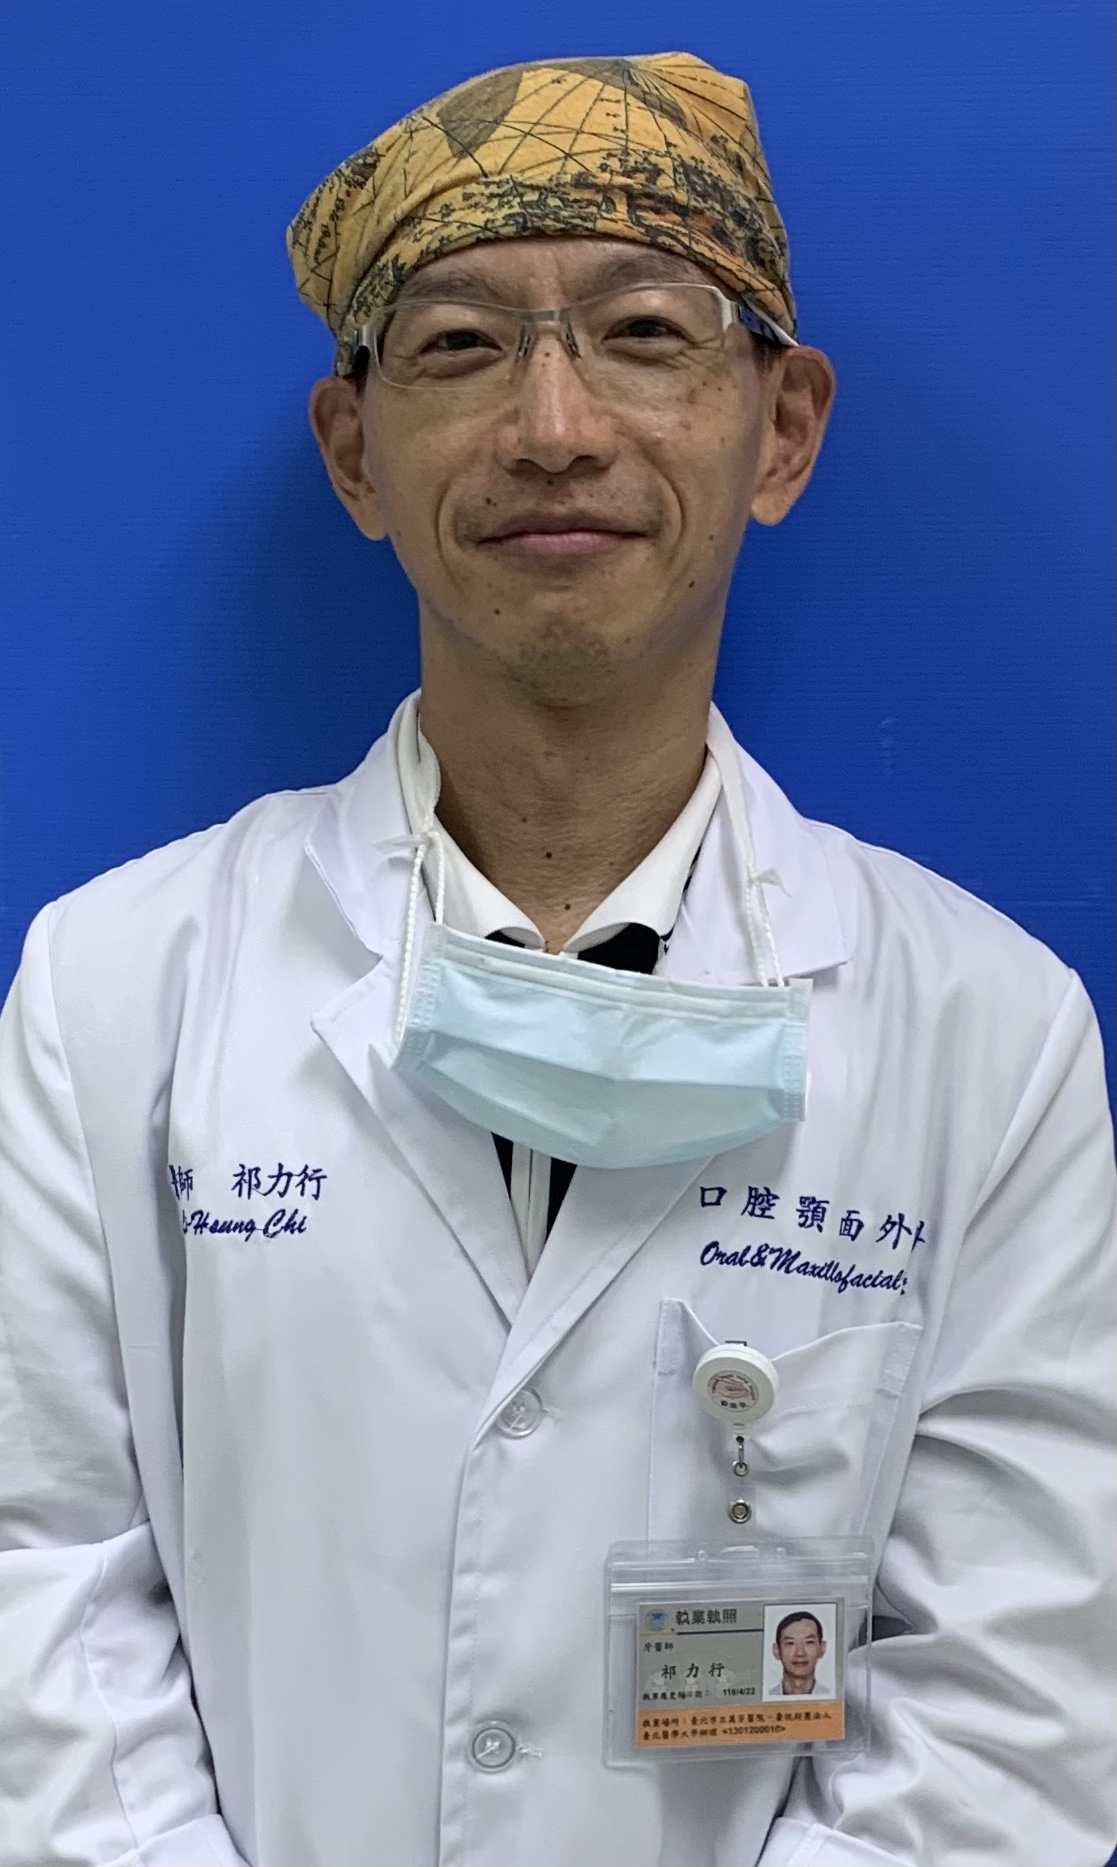
\includegraphics[height=40mm]{IMG_5507_Tex_portrait_TMWH.jpg}
\end{wrapfigure}

\noindent
Director (April 2021 - present)\\
Division of Oral and Maxillofacial Surgery, Department of Dentistry, Taipei Municipal Wanfang Hospital\\[4mm]
Attending physician (Jan. 2002 - present)\\
Division of Oral and Maxillofacial Surgery, Department of Dentistry,
Taipei Medical University Hospital\\
Taipei, Taiwan\\

\vspace{5mm}
% --- Start the two-column table storing the main content ---

% Set spacing between columns
\setlength{\tabcolsep}{8pt}

% Set the width of each column
\begin{longtable}{p{1.3in}p{4.8in}}

% --- Section: Research interests ---

\nohyphens{\color{OliveGreen}{Research interests}}
& Biostatistics with R/Python/C++ for survival analyses and deep learning, biomedical informatics; cancer research in vitro and in vivo; mindfulness meditation, laser acupuncture; forensic medicine. \\
& \\

% --- Section: Education ---
% my dissertation:
%1. Chi L-H. Global Transcriptomics and Proteomics Analyses for Biomarker Identification and Validation in Head and Neck Squamous Cell Carcinoma. Published online 2022/01/22.

\color{OliveGreen}{Education} 
& \textbf{Taipei Medical University and Academia Sinica} \hfill Taipei, Taiwan \\ 
& The Ph.D. Program for  Translational Medicine \hfill Feb. 2013 -- Feb. 2022 \\
& Mentors: Professors Yu-Chuan (Jack) Li, Michael Hsiao, Alex T.H Wu. \\
& \\

& \textbf{Taipei Medical University} \hfill Taipei, Taiwan \\
& MS in Biomedical Informatics \hfill Sep. 2011 -- Jan. 2013\\
& Mentor: Professor Yu-Chuan (Jack) Li.\\ % {\it GPA: X.YZ.}\\
& \\
% Yu-Chuan Jack Li M.D., Ph.D., FACMI

& \textbf{Taipei Medical University} \hfill Taipei, Taiwan \\
& BS in Dentistry \hfill Sep. 1988 -- Jun. 1994 \\
& \\% Mentors: Professors E, F. {\it GPA: X.YZ.}\\
& \\

% --- Uncomment the next few lines if you want to include some courses ---
%& \textbf{Selected coursework}
%\begin{itemize}[noitemsep,leftmargin=*]
%\item \underline{Relevant subject 1}: Course 1, Course 2, Course 3, Course 4
%\item \underline{Relevant subject 2}: Course 1, Course 2, Course 3, Course 4
%\end{itemize} \\

% --- Section: Awards, scholarships, etc. ---
% --- Note: section title is spread over two lines ---

{\color{OliveGreen}{Honors and award}} 
& Best Paper Presentation Award - 3rd Prize, at Translational Medicine
Program Retreat (Academia Sinica, Taiwan) \hfill 2017\\
%{\color{OliveGreen}{scholarships}} 
%& Name of award 2 (Organization that gave you the award)\hfill 2019 \\
%& Name of award 3 (Organization that gave you the award) \hfill 2018 \\
%& \\



% --- Section: Industry experience ---

%{\color{OliveGreen}{Industry experience}} 
%& {\textbf{Name of company,}} Division of company \hfill City, State\\
%& Title of job or internship \hfill Summer 2020 \\
%& Description of your responsibilities. Integer pretium semper justo. Proin risus. Nullam id quam. Nam neque. Phasellus at purus et lib ero lacinia dictum. Sed dolor lacus, imperdiet non, ornare non, commodo eu, neque.\\
%& \\
 
%& {\textbf{Name of company,}} Division of company \hfill City, State\\
%& Title of job or internship \hfill Summer 2020 \\
%& Description of your responsibilities. Integer pretium semper justo. Proin risus. Nullam id quam. Nam neque. Phasellus at purus et lib ero lacinia dictum. Sed dolor lacus, imperdiet non, ornare non, commodo eu, neque.\\
%& \\

% --- Section: Talks and tutorials ---

{\color{OliveGreen}{Presentation}} 
& \textbf{A Transcriptomic Analysis of Head and Neck Squamous Cell Carcinomas for Prognostic Indications} \hfill Sep. 10, 2021 \\
& The 8th Annual Academic Achievements Presentation of Translation Medicine Degree Program \\
& \\

& \textbf{Global Proteomics-based Identification
and Validation of Thymosin Beta-4 X-Linked as a Prognostic Marker for Head
and Neck Squamous Cell Carcinoma} \hfill Sep. 6, 2017 \\
& The 4th Translational Medicine
Program Retreat, Taipei, Taiwan. \\
& \\

& \textbf{Silencing JARID1B Suppresses
Oncogenicity, Stemness and Increases Radiation Sensitivity in Head and
Neck Squamous Cell Carcinoma} \hfill Sep. 4, 2015 \\
& The 2nd Annual Retreat of the
Translational Medicine Degree Program, Kaohsiung, Taiwan. \\
& \\


& \textbf{Glucose Transporter 4, encoded by gene
SLC2A4, as a Prognostic Marker for Head and Neck Squamous Cell
Carcinoma} \hfill Sep. 19, 2014 \\
& The 1st Annual Retreat of the Translational Medicine Degree Program, Taipei, Taiwan. \\
& \\


& \textbf{A Summary of International Partnership for Health Informatics Education} \hfill  2012 \\
& IPHIE2012 Master
class training of Health Informatics, University Of Minnesota, Twin
Cities, MN, U.S.A. \\
& \\

& \textbf{Recurrent Ameloblastic Carcinoma ex
Ameloblastoma of Maxilla - A case report} \hfill June 2005 \\
& ICOMS – 17th International
Conference on Oral and Maxillofacial Surgery, Vienna, Austria. \\
& \\



% --- Section: Various skills (programming, software, languages, etc.) ---

{\color{OliveGreen}{Skills}} 
& \textbf{Programming}\\
& Proficient in: R, Python/PyTorch. \\
& Familiar with: Matlab, SAS, C++. \\
& \\

& \textbf{Languages} \\
& Chinese, English (fluent) \\
& \\

% --- Section: Service and outreach ---

\color{OliveGreen}{Service and outreach by TMU} % Africa
& \textbf{Royal Health Mission in the Kingdom of Eswatini, southern Africa} \hfill Sep. 2014 -- Sep. 2019 \\
& attending physician working at the Manzana Clinic. \\
& \\

& \textbf{Missão Médica de Taiwan em São Tomé e Príncipe, west Africa} \hfill Nov. 2010 -- Jan. 2012 \\
& attending physician working at hospital central em São Tomé e Príncipe. \\
& \\

& \textbf{Taiwan Medical Mission in the Kingdom of Swaziland, southern Africa} \hfill May 2009 -- Nov. 2010 \\
& attending physician working at the Mbabane Government Hospital. \\
& \\

% --- Section: Professional society memberships ---
% --- Note: section title is spread over two lines ---

\nohyphens{\color{OliveGreen}{Professional memberships}}
& {\textbf{Taiwanese Association of Oral and Maxillofacial Surgeons (TAOMS)}} \hfill Jan. 2002 -- Present \\
%{\color{OliveGreen}{memberships}} 
& Taiwan Society of Forensic Medicine (TSFM) \hfill 2022-\\ 
& Taiwan Biophysics Society \hfill 2014-\\ 
& Taiwan Society for Integration of Chinese and Western Medicine (CWM) \hfill 2019-\\
& Chinese Medical Association of Acupuncture (CMAA, Taiwan) \hfill 2019- \\
& \\

% --- Section: Other interests/hobbies ---

%\nohyphens{\color{OliveGreen}{Manuscript under review}}
%& \textbf{A Global Genome-Wide Scan with Optimal Cutoff Mining for Emerging Biomarkers in Head and Neck Squamous Cell Carcinoma} \\
%& Chi, Li-Hsing and Wu, Alexander T H and Hsiao, Michael and Li, Yu-Chuan Jack.\\
%& \textit{Research Square [Preprint Server], 2020}\\
%& \\

%\pagebreak

\nohyphens{\color{OliveGreen}{References}} 
& Dr. Bou-yue Pemg, D.D.S., M.S.\\
& Director\\
%Attending physician and specialist,
& Oral and Maxillofacial Surgery, Department of Dentistry,
Taipei Medical University Hospital,
Taipei, Taiwan\\
& E-mail: pemg@tmu.edu.tw\\[0.5cm]


& Professor Yu-Chuan Jack Li, M.D.,  Ph.D.\\
& Professor\\
& Professional Master Program for Artificial Intelligence in Medicine, Taipei Medical University,
Taipei, Taiwan\\
& E-mail: jack@tmu.edu.tw\\[0.5cm]


& Professor Michael Hsiao, D.V.M., Ph.D.\\
& Research Fellow\\
& Genomics Research Center, 
Academia Sinica, Taipei, Taiwan\\
& E-mail: mhsiao@gate.sinica.edu.tw\\[1.35cm]

%\clearpage
& Dr. Alex T.H Wu, Ph.D.\\
& Associate Professor\\
& Graduate Program in Translational Medicine,
College of Medical Science and Technology,
Taipei Medical University,
Taipei, Taiwan\\
& E-mail: chaw1211@tmu.edu.tw\\




\end{longtable}


% --- Section: Publications ---
\nohyphens{\color{OliveGreen}{Publications}} 
\printbibliography[heading=none] %, 
%\printbibliography[heading=subbibliography, notkeyword=donotinclude]

%\bibliography{Tex_publications_since2002.bib} % lib.bib file inside ref folder
%\bibliographystyle{model1-num-names}
% model1-num-names
% apacite
\nocite{*}

% --- End of CV! ---
%\end{document}
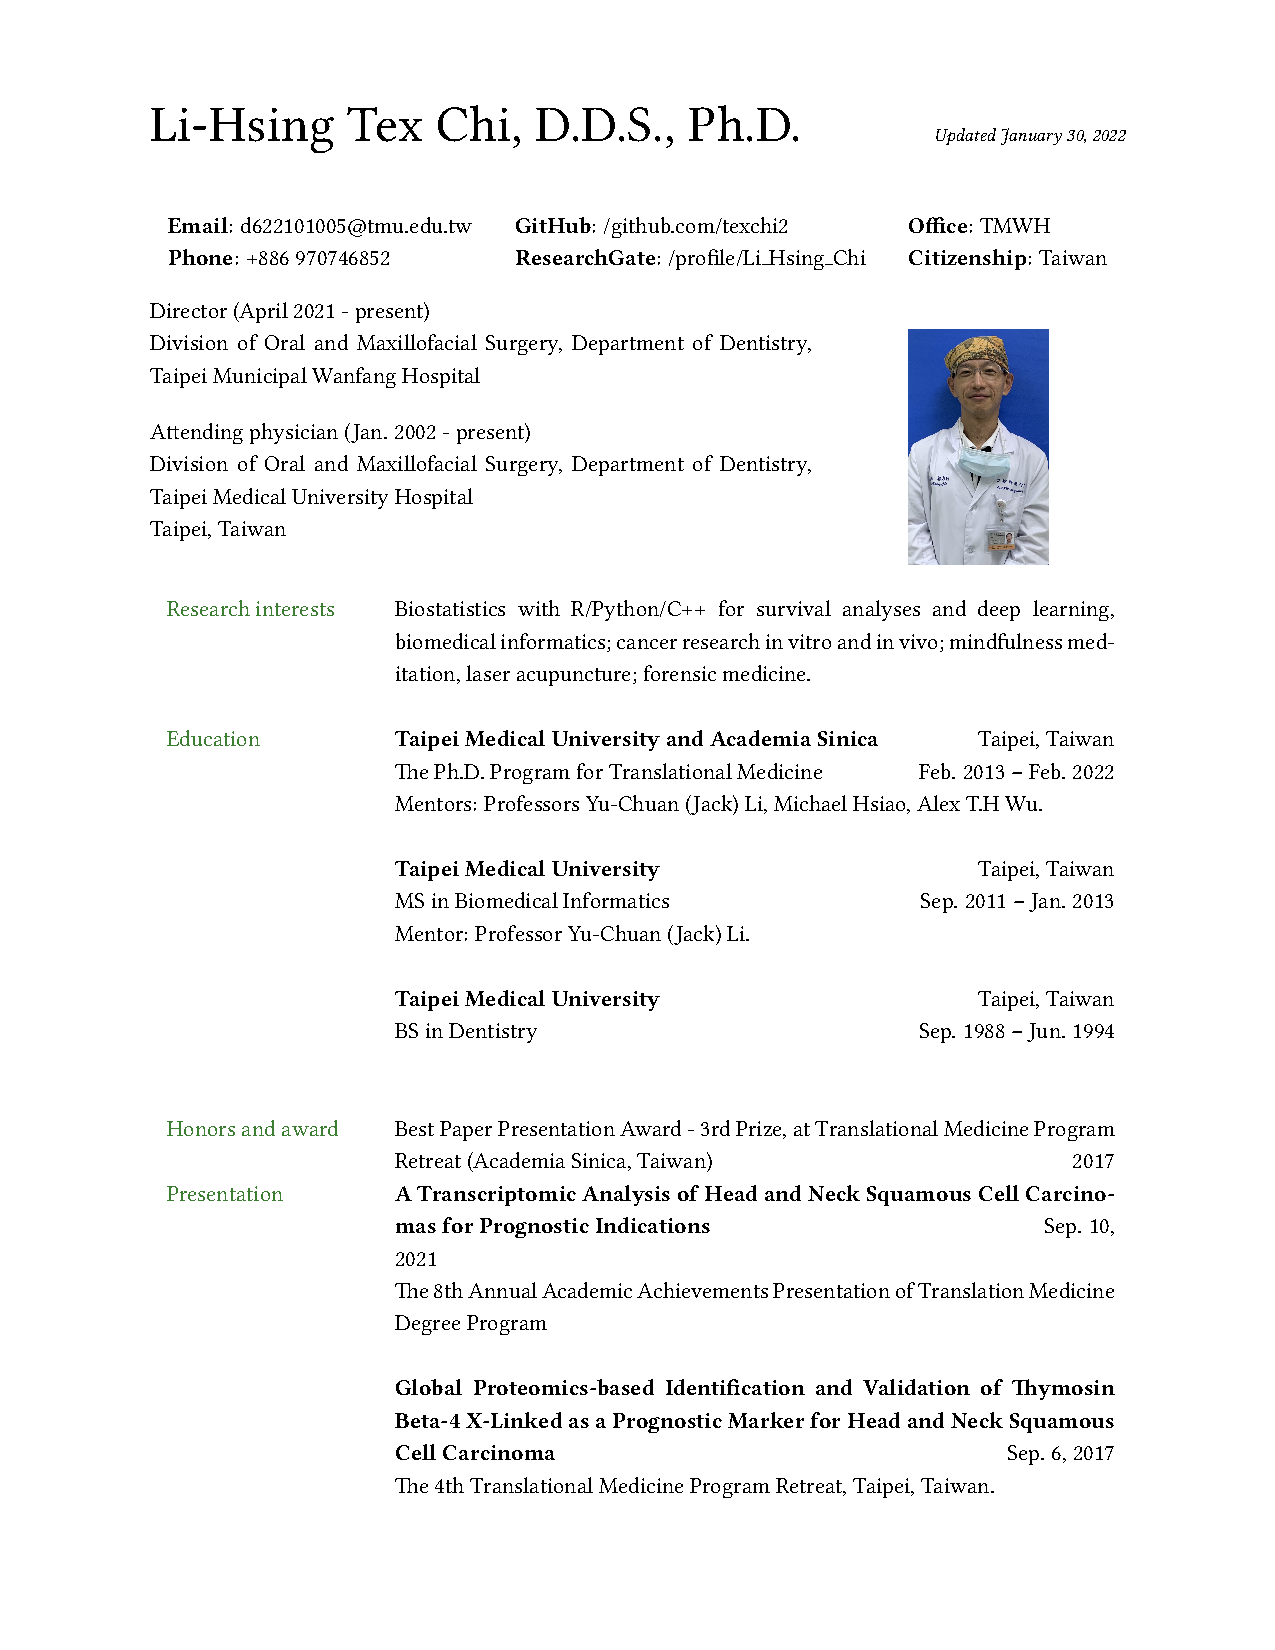
\includepdf[pages=-]{AcademicCV_Li_Hsing_Chi2022.pdf}

\end{letter}



\end{document}